\begin{frame}<5>[label=sem]{Structural equation models}
  \small
  \vspace*{-0.2cm}\hspace*{-1cm}\begin{tikzpicture}
    \node[draw=black,inner sep=2pt,anchor=west,text width=5cm] (envir03) at (0, 0) {\scriptsize Ecology disadvantages minority and small businesses};
    \node[draw=black,inner sep=2pt,anchor=west,text width=5cm] (envir05) at (0, 0.7) {\scriptsize I am concerned about global warming};
    \node[draw=black,inner sep=2pt,anchor=west,text width=5cm] (envir06) at (0, 1.6) {\scriptsize Actions and decision making are needed to limit greenhouse gas emissions};

    \node[draw=black,inner sep=2pt,anchor=west,text width=5cm] (mobil12) at (0, 3) {\scriptsize It is very important to have a beautiful car};
    \node[draw=black,inner sep=2pt,anchor=west,text width=5cm] (mobil13) at (0, 3.9) {\scriptsize With my car I can go wherever and whenever};
    \node[draw=black,inner sep=2pt,anchor=west,text width=5cm] (mobil14) at (0, 4.8) {\scriptsize When I take the car I know I will be on time};

    \node[draw=black,inner sep=2pt,anchor=west,text width=5cm] (income) at (0, 5.6) {\scriptsize Income};
    \node[draw=black,inner sep=2pt,anchor=west,text width=5cm] (howner) at (0, 6) {\scriptsize Homeowner};
    \node[draw=black,inner sep=2pt,anchor=west,text width=5cm] (rooms) at (0, 6.4) {\scriptsize Number of rooms in home};

    \node[draw=black,inner sep=2pt,rounded corners=0.2cm,anchor=west] (env) at (6.5, 0.7) {Environmental attitude};
    \node[draw=black,inner sep=2pt,rounded corners=0.2cm,anchor=west] (car) at (6.5, 3.9) {Pro-car attitude};
    \node[draw=black,inner sep=2pt,rounded corners=0.2cm,anchor=west] (ses) at (6.5, 5.7) {Socioeconomic status};

    \draw[->] (env.west) -- node[midway,below,sloped] (m1) {\tiny \only<5->{-0.39***}} (envir03.east);
    \draw[->] (env.west) -- node[midway,sloped] (m2) {\tiny \only<5->{0.95***}} (envir05.east);
    \draw[->] (env.west) -- node[midway,above,sloped] (m3) {\tiny \only<5->{1}} (envir06.east);

    \draw[->] (car.west) -- node[midway,below,sloped] (m4) {\tiny \only<5->{1}} (mobil12.east);
    \draw[->] (car.west) -- node[midway,sloped] (m5) {\tiny \only<5->{1.27***}} (mobil13.east);
    \draw[->] (car.west) -- node[midway,above,sloped] (m6) {\tiny \only<5->{2.76***}} (mobil14.east);

    \draw[->] (ses.west) -- node[midway,below,sloped] (m7) {\tiny \only<5->{8.08***}} (income.east);
    \draw[->] (ses.west) -- node[midway,sloped] (m8) {\tiny \only<5->{1}} (howner.east);
    \draw[->] (ses.west) -- node[midway,above,sloped] (m9) {\tiny \only<5->{5.93***}} (rooms.east);

    \draw[<->] (car.south) -- node[midway,above,sloped] (cor) {\tiny \only<5->{-0.07***}} (env.north);

    \only<1,3->{
      \node[draw=black,inner sep=2pt,anchor=west] (ncars) at (11, 3.9) {Number of cars owned};
      \node[draw=black,inner sep=2pt,anchor=west] (pass) at (11, 2) {Transit pass};

      \draw[->] (ses.south) -- node[midway,above,sloped] (s1) {\tiny \only<5->{-0.41***}} (car.north);
      \path[->,bend left] ([xshift=1cm]ses.south) edge node[pos=0.3,above,sloped] (s2) {\tiny \only<5->{0.49**}} ([xshift=1cm]env.north);

      \draw[->] (env.east) -- node[pos=0.3,above,sloped] (s3) {\tiny \only<5->{-0.01}} ([yshift=-3pt]ncars.west);
      \draw[->] (car.east) -- node[pos=0.2,above,sloped] (s4) {\tiny \only<5->{0.44***}} (ncars.west);
      \draw[->] (ses.east) -- node[midway,above,sloped] (s5) {\tiny \only<5->{1.90***}} ([yshift=3pt]ncars.west);

      \draw[->] (env.east) -- node[midway,below,sloped] (s6) {\tiny \only<5->{0.01}} ([yshift=-3pt]pass.west);
      \draw[->] (car.east) -- node[pos=0.3,above,sloped] (s7) {\tiny \only<5->{-0.36***}} (pass.west);
      \draw[->] (ses.east) -- node[pos=0.85,above,sloped] (s8) {\tiny \only<5->{0.47***}} ([yshift=3pt]pass.west);
      \draw[->] (ncars.south) -- node[midway,above,sloped] (s9) {\tiny \only<5->{-0.13***}} (pass.north);
    }

    % force alignment
    \path (envir06.west) -- +(180:1cm);
    \path (envir06.north) -- +(90:1cm);

    \only<4-5>{
      \draw[<-] (envir06.west) -- node[midway,above] {\tiny \only<5->{0.19}} +(180:0.75cm) node[text=black,anchor=east] {\footnotesize$\delta$};
      \draw[<-] (envir05.west) -- node[midway,above] {\tiny \only<5->{0.77}} +(180:0.75cm) node[text=black,anchor=east] {\footnotesize$\delta$};
      \draw[<-] (envir03.west) -- node[midway,above] {\tiny \only<5->{1.47}} +(180:0.75cm) node[text=black,anchor=east] {\footnotesize$\delta$};
      \draw[<-] (mobil12.west) -- node[midway,above] {\tiny \only<5->{1.39}} +(180:0.75cm) node[text=black,anchor=east] {\footnotesize$\delta$};
      \draw[<-] (mobil13.west) -- node[midway,above] {\tiny \only<5->{0.70}} +(180:0.75cm) node[text=black,anchor=east] {\footnotesize$\delta$};
      \draw[<-] (mobil14.west) -- node[midway,above] {\tiny \only<5->{0.53}} +(180:0.75cm) node[text=black,anchor=east] {\footnotesize$\delta$};
      \draw[<-] (howner.west) -- node[midway,above] {\tiny \only<5->{0.17}} +(180:0.75cm) node[text=black,anchor=east] {\footnotesize$\delta$};
      \draw[<-] (income.west) -- node[midway,above] {\tiny \only<5->{5.11}} +(180:0.75cm) node[text=black,anchor=east] {\footnotesize$\delta$};
      \draw[<-] (rooms.west) -- node[midway,above] {\tiny \only<5->{1.23}} +(180:0.75cm) node[text=black,anchor=east] {\footnotesize$\delta$};

      \draw[<-] (ncars.north) -- node[midway,above,sloped] {\tiny \only<5->{0.36}} +(90:0.75cm) node[text=black,anchor=south] {\footnotesize$\delta$};
      \draw[<-] (pass.south) -- node[midway,above,sloped] {\tiny \only<5->{0.20}} +(270:0.75cm) node[text=black,anchor=north] {\footnotesize$\delta$};

      \draw[<-] (env.south) -- node[midway,above,sloped] {\tiny \only<5->{0.46}} +(270:0.75cm) node[text=black,anchor=north] {\footnotesize$\zeta$};
      % This one is basically zero, and there shouldn't be a structural error here anyhow because there are no predictors of this variable - see p30ff of Bowen and Guo
      %\draw[<-] (ses.east) -- node[midway,above,sloped] {\tiny \only<5->{0.02}} +(15:0.75cm) node[text=black,anchor=west] {\footnotesize$\zeta$};
      \draw[<-] ([xshift=-1em]car.south) -- node[midway,above,sloped] {\tiny \only<5->{0.11}} +([xshift=-1em]270:0.75cm) node[text=black,anchor=north] {\footnotesize$\zeta$};
    }

    \only<9>{
      \node[text=red,anchor=west] (lat) at (11, 5) {Latent variables};
      \draw[->,red] (lat) -- (env);
      \draw[->,red] (lat) -- (car);
      \draw[->,red] (lat) -- (ses);
    }

    \only<10-11>{
      \node[text=red,anchor=west] (mpart) at (6.5, 6.3) {Measurement part};
      \path[->,red,bend left] (mpart.south) edge (m1);
      \path[->,red,bend left] (mpart.south) edge (m2);
      \path[->,red,bend left] (mpart.south) edge (m3);
      \path[->,red,bend left] (mpart.south) edge (m4);
      \path[->,red,bend left] (mpart.south) edge (m5);
      \path[->,red,bend left] (mpart.south) edge (m6);
      \path[->,red,bend left] (mpart.south) edge (m7);
      \path[->,red,bend left] (mpart.south) edge (m8);
      \path[->,red,bend left] (mpart.south) edge (m9);
      \path[->,red,bend left] (mpart.south) edge (cor);
    }

    \only<11>{
      \node[text=red,anchor=west] (corlab) at (5.5, 3) {Correlation};
      \path[->,red] (corlab) edge (cor);
    }

    \only<12>{
      \node[text=red,anchor=west] (slab) at (11, 1) {Structural part};
      \path[->,red,bend right] (slab.north) edge (s1);
      \path[->,red,bend right] (slab.north) edge (s2);
      \path[->,red,bend right] (slab.north) edge (s3);
      \path[->,red,bend right] (slab.north) edge (s4);
      \path[->,red,bend right] (slab.north) edge (s5);
      \path[->,red,bend right] (slab.north) edge (s6);
      \path[->,red,bend right] (slab.north) edge (s7);
      \path[->,red,bend right] (slab.north) edge (s8);
      \path[->,red,bend right] (slab.north) edge (s9);
    }

    \only<7-8>{
      \draw[->,red] (ses.east) -- node[midway,below,sloped,text=red] (s5) {\small Direct effect} ([yshift=3pt]ncars.west);
    }

    \only<8>{
      \draw[->,red] (ses.south) -- coordinate[midway] (ind1) (car.north);
      \draw[->,red] (car.east) -- coordinate[midway] (ind2) (ncars.west);
      \path (ind1) -- node[midway,sloped,text=red] {Indirect effect} (ind2);
    }

    \only<5->{\node (sigstars) at (11, 0) {\tiny * = p < 0.05, ** = p < 0.01, *** = p < 0.001};}

  \end{tikzpicture}\\
  \hfill\tiny Data: \textcite{bierlaire_mode_2018}
\end{frame}
\againframe<1-2>{sem}

\begin{frame}{Structural equation models}
  % https://tex.stackexchange.com/questions/44449
  \newcommand*\grayout{black!40}
  \small
  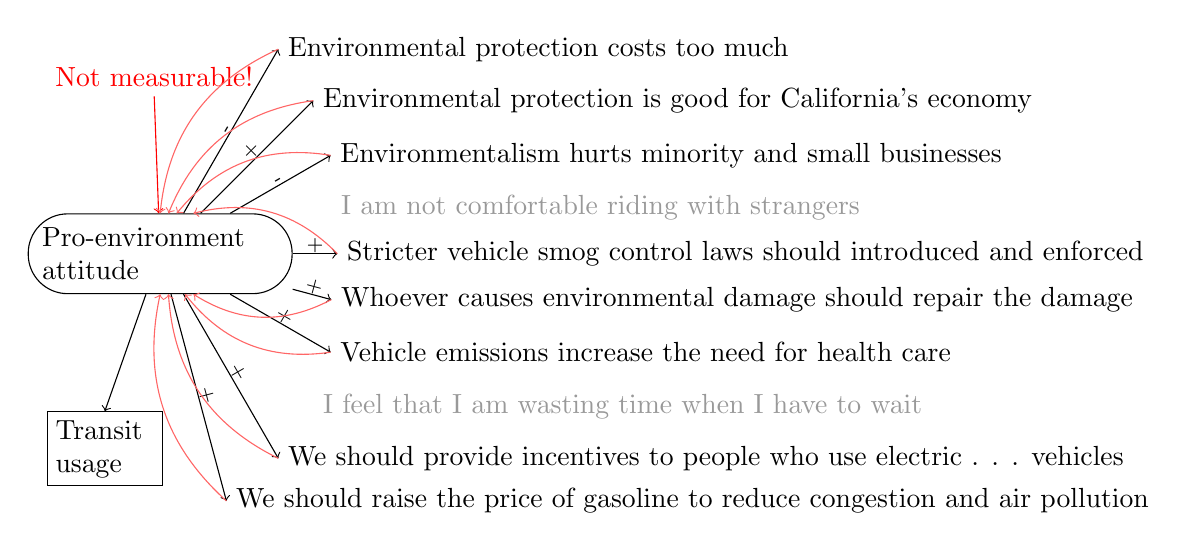
\begin{tikzpicture}
    \node[draw=black,inner sep=5pt,rounded corners=0.5cm,text width=3cm,anchor=east] (attitude) at (3, 5) {\normalsize  Pro-environment attitude};

    \draw[->] ([xshift=-2em]attitude) -- +(270:2cm) node[text=black,anchor=north,text width=1.25cm,inner sep=3pt,draw=black] { Transit usage };


    \draw[<-,color=red] (attitude) -- +([xshift=-0.5ex] 90:2cm) node[text=red,anchor=south] {Not measurable!};


    \node[anchor=west,text=black] (cost) at ([shift=({60:3cm})]attitude) {Environmental protection costs too much};
    \node[anchor=west,text=black] (econ) at ([shift=({45:2.75cm})]attitude) {Environmental protection is good for California’s economy};
    \node[anchor=west,text=black] (hurtssb) at ([shift=({30:2.5cm})]attitude) {Environmentalism hurts minority and small businesses};
    \node[anchor=west,text=\grayout] (strangers) at ([shift=({15:2.25cm})]attitude) {I am not comfortable riding with strangers};
    \node[anchor=west,text=black] (smog) at ([shift=({0:2.25cm})]attitude) {Stricter vehicle smog control laws should  introduced and enforced};
    \node[anchor=west,text=black] (damage) at ([shift=({345:2.25cm)})]attitude) {Whoever causes environmental damage should repair the damage};
    \node[anchor=west,text=black] (emissions) at ([shift=({330:2.5cm})]attitude) {Vehicle emissions increase the need for health care};
    \node[anchor=west,text=\grayout] (time) at ([shift=({315:2.75cm})]attitude) {I feel that I am wasting time when I have to wait};
    \node[anchor=west,text=black] (ev) at ([shift=({300:3cm})]attitude) {We should provide incentives to people who use electric . . . vehicles};
    \node[anchor=west,text=black] (raisegas) at ([shift=({285:3.25cm})]attitude) {We should raise the price of gasoline to reduce congestion and air pollution};

    \draw[->] (attitude) -- (cost.west)
      node[yshift=-0.75ex, midway, above, sloped] {\scriptsize -};
    \draw[->] (attitude) -- (econ.west)
        node[yshift=-0.75ex, midway, above, sloped] {\scriptsize +};
    \draw[->] (attitude) -- (hurtssb.west)
        node[yshift=-0.75ex, midway, above, sloped] {\scriptsize -};
    \draw[->] (attitude) -- (smog.west)
        node[yshift=-0.75ex, midway, above, sloped] {\scriptsize +};
    \draw[->] (attitude) -- (damage.west)
        node[yshift=-0.75ex, midway, above, sloped] {\scriptsize +};
    \draw[->] (attitude) -- (emissions.west)
        node[yshift=-0.75ex, midway, above, sloped] {\scriptsize +};
    \draw[->] (attitude) -- (ev.west)
        node[yshift=-0.75ex, midway, above, sloped] {\scriptsize +};
    \draw[->] (attitude) -- (raisegas.west)
        node[yshift=-0.75ex, midway, above, sloped] {\scriptsize +};


    \path[->,color=red!60,bend right] (cost.west) edge ([xshift=0pt]attitude.north);
    \path[->,color=red!60,bend right] (econ.west) edge ([xshift=3pt]attitude.north);
    \path[->,color=red!60,bend right] (hurtssb.west) edge ([xshift=6pt]attitude.north);
    \path[->,color=red!60,bend right] (smog.west) edge ([xshift=12pt]attitude.north);
    \path[->,color=red!60,bend left] (damage.west) edge ([xshift=12pt]attitude.south);
    \path[->,color=red!60,bend left] (emissions.west) edge ([xshift=9pt]attitude.south);
    \path[->,color=red!60,bend left] (ev.west) edge ([xshift=3pt]attitude.south);
    \path[->,color=red!60,bend left] (raisegas.west) edge ([xshift=0pt]attitude.south);


  \end{tikzpicture}

  {\tiny Based on \textcite{kitamura_micro-analysis_1997}}
\end{frame}
\againframe<2->{sem}

\begin{frame}{Structural equation models}
  \begin{itemize}
    \item SEMs need a strong basis in theory
    \item Correlation (still) does not imply causation (even when there are arrows!)
    \begin{itemize}
      \item SEMs test whether data is consistent with theoretical causal structures \autocite{bollen_eight_2013}
    \end{itemize}
    \item Authors should test multiple SEMs \autocite{bowen_structural_2012}
    \item There are many ways to evaluate model fit \autocite[see][]{bowen_structural_2012}
    % \begin{itemize}
    %   \item For this class, assume models fit well unless authors state otherwise
    % \end{itemize}
  \end{itemize}
\end{frame}

% Comment out for publication
% \begin{frame}{Recording structural equation models}
%   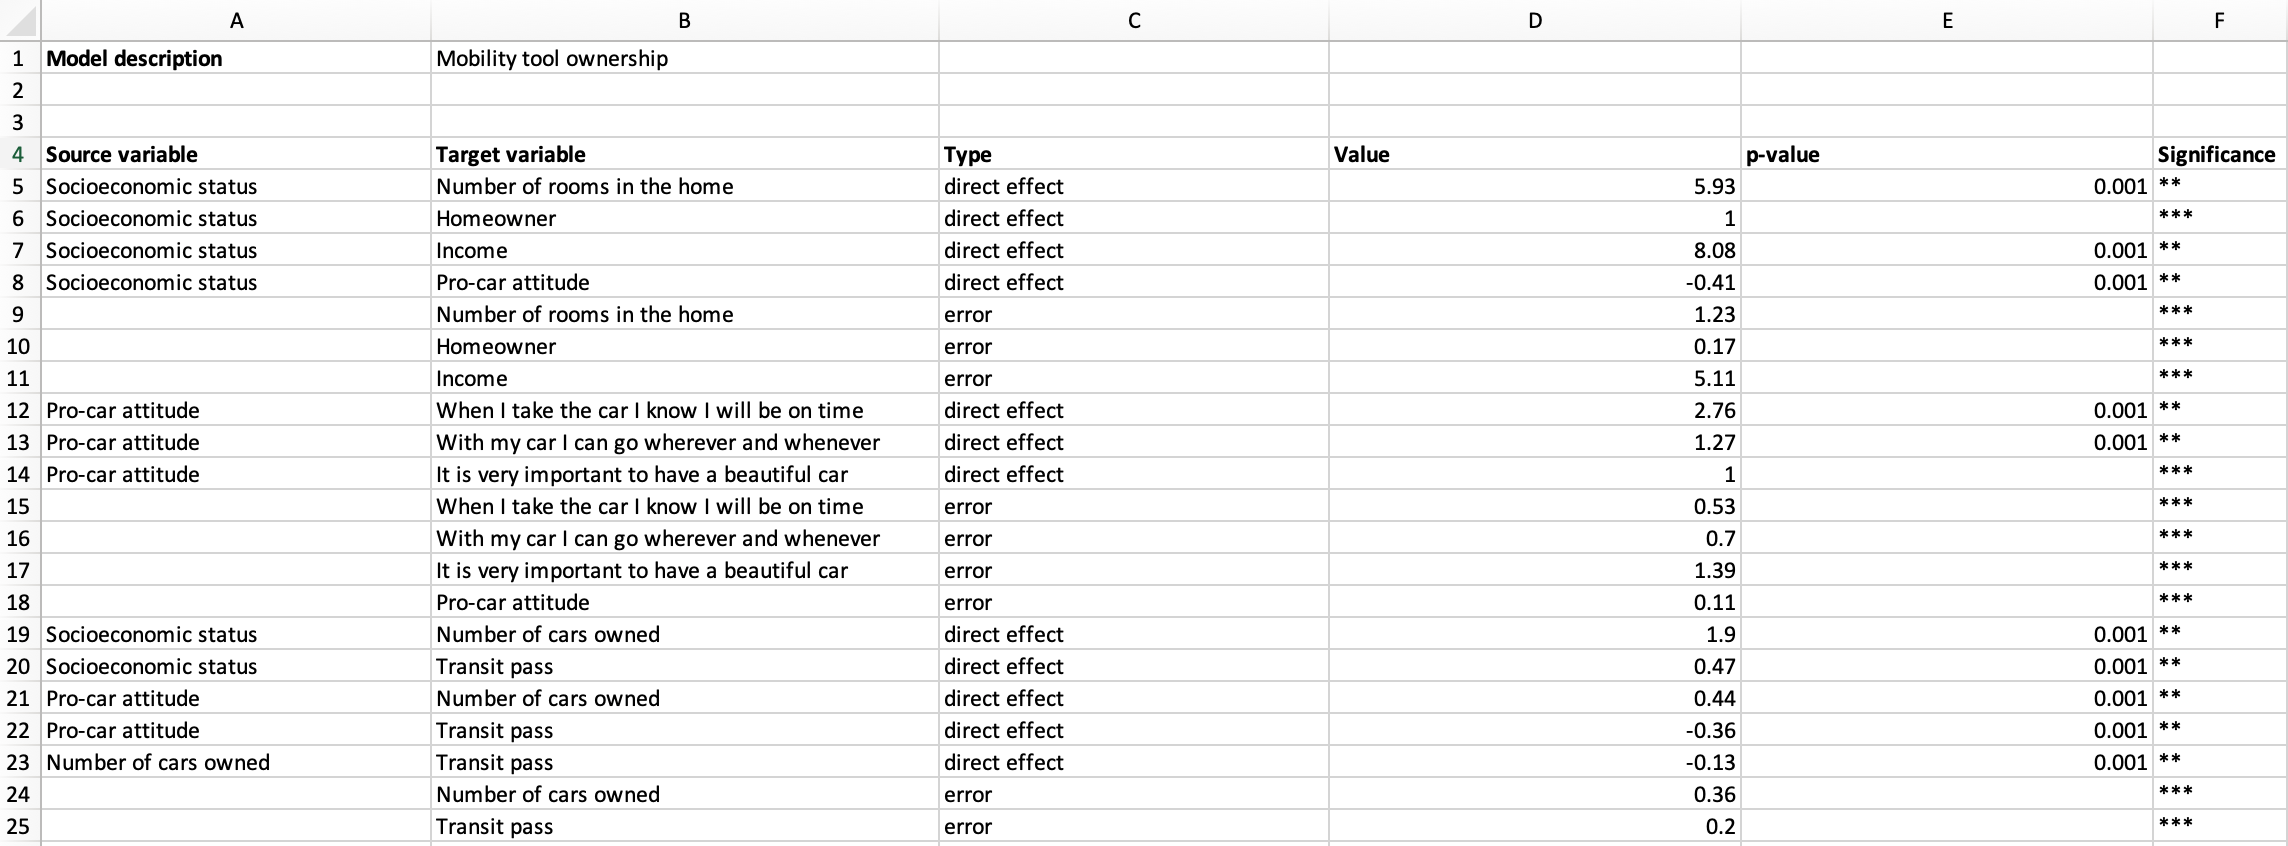
\includegraphics[width=\textwidth]{img/sem_excel.png}
% \end{frame}

\begin{frame}{Structural equation models: table form}
  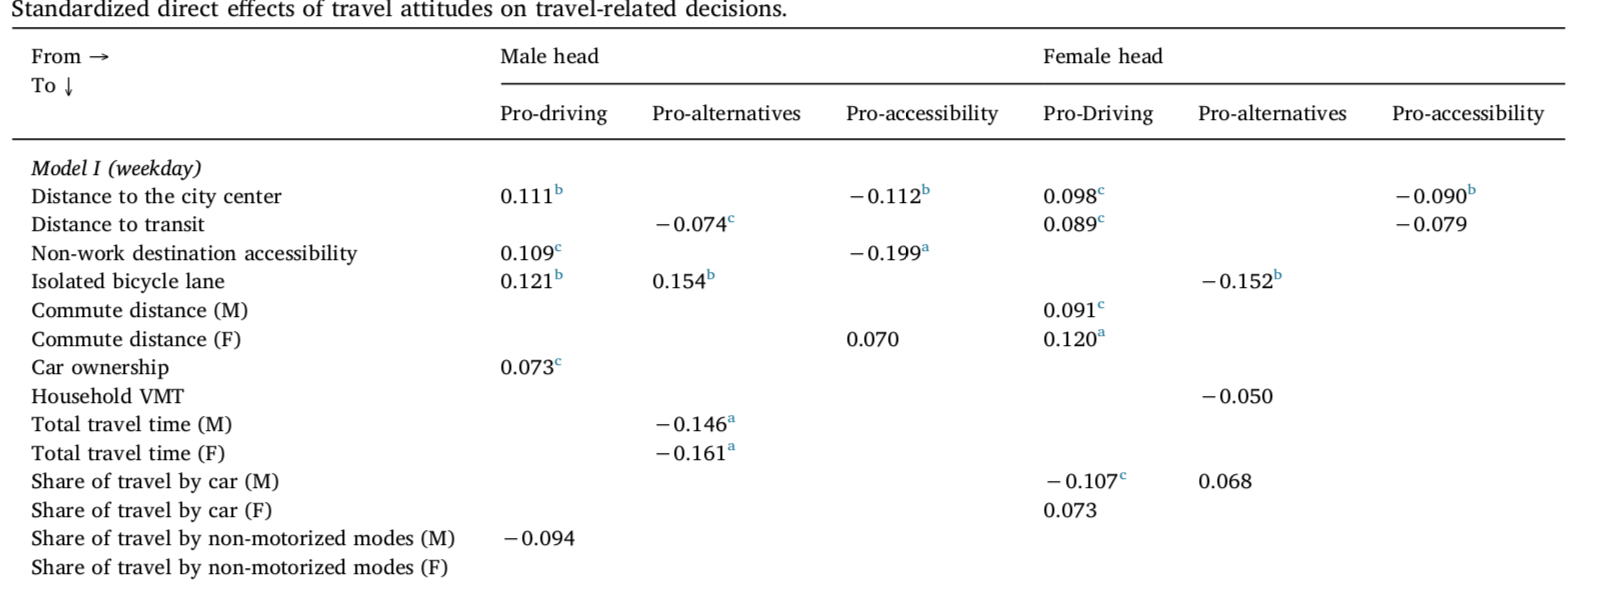
\includegraphics[width=\textwidth]{img/guan_sem.png}\\
  {\tiny \textcite{guan_residential_2019}}
\end{frame}
